\chapter{Quantum Networking With an Elementary Operating System}
\label{chp:qnodeos}

\begin{abstract}
Chapter abstract.
\end{abstract}

\noindent
\note{To be precise, this chapter is extracted from sections 5 (Implementation), 6 (Evaluation), 7
(Related Work) and 8 (Discussion) from the \acrshort{qnodeos} paper. In addition, the description of
the test applications was expanded to add more context.}

\blfootnote{
    This chapter is based on the preprint \fullcite{delledonne_2023_qnodeos_noprint}. \note{Add
    proper link to arXiv when submitted}
}

\newpage

% \lettrine{T}{...}

Some information and context about evaluation strategy and goals.

\section{Implementation}
\label{sec:qnodeos:implementation}

\Cref{fig:node-deployment} outlines software and hardware implementation of \acrshort{qnodeos} and
the whole node system. \acrshort{qnodeos} is implemented in C++ on top of FreeRTOS, a tiny operating
system for microcontrollers~\cite{freertos}. The stack runs on a dedicated MicroZed~\cite{microzed}
--- an off-the-shelf platform based on the Zynq-7000 SoC, which hosts two ARM Cortex-A9 processing
cores, of which only one is used, clocked at \qty{667}{\MHz}. \acrshort{qnodeos} connects to peer
\acrshort{qnodeos} systems via \acrshort{tcp} over a Gigabit Ethernet interface. For the
\acrshort{qdevice}, we replicated the setup used for \cref{chp:netstack}, which mainly consists of:
%
\begin{enumerate*}[label=(\arabic*)]
    \item an ADwin-Pro II~\cite{adwin} acting as the main orchestrator of the setup;
    \item a series of subordinate devices responsible for qubit control, including laser pulse
          generators and optical readout circuits;
    \item the quantum physical device, based on \acrshort{nv} centers, counting one single
          (communication) qubit for each node.
\end{enumerate*}
The \acrshort{qdevice} is where the time-critical qubit control lies. \acrshort{qnodeos} interfaces
with the \acrshort{qdevice}'s ADwin-Pro II through a \qty{12.5}{\MHz} \acrshort{spi} interface, used
to exchange 4-byte control messages at a rate of \qty{50}{kHz}. Finally, the host layer is a Python
runtime executing on a general-purpose 4-core desktop machine running Linux. The host machine
connects to \acrshort{qnodeos} via \acrshort{tcp} over the same Gigabit Ethernet interface that
\acrshort{qnodeos} uses to connect to its peers (average ping \acrshort{rtt} of \qty{0.1}{\ms}), and
sends application registration requests and quantum code blocks over this interface (\num{10} to
\num{1000} bytes, depending on the length of the block). \Cref{app:qnodeos} provides additional
details on the implementation of the components of \acrshort{qnodeos} and their interfaces.
Moreover, the specification of the interface to the \acrshort{qdevice} is given in
\cref{app:qdevice}. 

We implemented \acrshort{qnodeos} on top of FreeRTOS to avoid re-implementing standard \acrshort{os}
primitives like threads and network communication. FreeRTOS provides basic \acrshort{os}
abstractions like tasks, inter-task message passing, and the \acrshort{tcpip} stack. The FreeRTOS
kernel --- like any other standard \acrshort{os} --- cannot however directly manage the quantum
resources (qubits, entanglement requests and entangled pairs), and hence its task scheduler cannot
take decisions based on such resources. \acrshort{qnodeos} adds these capabilities and takes care of
the scheduling of quantum code blocks based on the status of the quantum resources.

\begin{figure}[t]
    \centering
    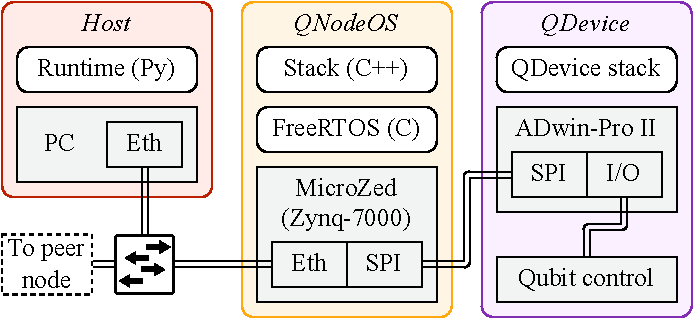
\includegraphics[width=0.6\linewidth]{figures/node-deployment.pdf}
    \caption{
        Node deployment overview. Our quantum network node consists of a desktop machine for the
        host runtime, a Zynq-7000 SoC for \acrshort{qnodeos}, and a series of digital and analog
        controllers for the \acrshort{qdevice}.
    }
    \label{fig:node-deployment}
\end{figure}

\section{Target Applications and Evaluation Goals}

First part of the ``Evaluation'' section from the \acrshort{qnodeos} paper, with a more extensive
explanation of the target applications (including multitasking), and an explanation of how each of
the apps, whilst conceptually simple, tests most functionalities of the \acrshort{os}.

\section{Results and Takeaways}

Second part of the ``Evaluation'' section from the \acrshort{qnodeos} paper.

\section{Related Work}
\label{sec:qnodeos:relwork}

Relative to quantum networking, a substantial amount of software and systems work happens in the
field of quantum computing. For example, operating systems for quantum computers (without networking
functionality) are under active development in research and industry~\cite{kong_2021_origin,
deltaflow_os}. Furthermore, extensive work exists on developing quantum computing
architectures~\cite{fu_2017_microarch, murali_2019_fullstack, bourassa_2021_blueprint}. In this
work, we have addressed new problems that arise specifically from the inclusion of quantum
networking which has not been considered at all in the aforementioned \acrshort{os}es and
publications.

Nevertheless, systems research in quantum networking has been growing as a field as well. In
particular, over the past several years there have been multiple proposals for quantum network
protocol stacks~\cite{van_meter_2013_repeaters, pirker_2019_quantum, dahlberg_2019_egp,
illiano_2022_quantum} and quantum network architectures~\cite{matsuo_2019_bootstrapping,
aguado_2020_enabling, li_2022_connectionless, diadamo_2022_packet, pouryousef_2022_overlay,
gu_2023_fendi, mandil_2023_packet}. One of the proposed network stacks has even been demonstrated
experimentally on a state-of-the-art two-node network in a lab~\cite{pompili_2022_experimental} ---
as detailed in \cref{chp:netstack} --- while the rest has only been validated in simulation.
However, these works heavily focus on the network protocol aspects and whilst some of them
acknowledge that the stacks will exist as a component in a bigger system, they do not tackle any of
the related issues, such as resource management or task scheduling.

Quantum network applications themselves have also been demonstrated on small networks in
laboratories~\cite{barz_2012_demonstration}. However, such demonstrations have always been \emph{ad
hoc}, and scripted through low-level experimental controls as their purpose was to demonstrate
hardware technology milestones rather than develop general systems for multiple users.

\section{Discussion}

\noindent
\note{Copy over from \acrshort{qnodeos} paper after experiments have been performed}

\printbibliography[heading=subbibintoc,title={References},notcategory=noprint]
